

\subsection{Camera Movement Tests}

In this section, camera parameters found by the FVR method are compared to ground truth data under various levels of noise. The Signal to Noise Ratio (SNR) metric is used to describe the noise added to the data prior to registration. A noise value of $x$\% means random noise was added in the range [$-0.5x$, $0.5x$]. Camera registration error is measured in centimetres and voxel error (the error in the phase correlation volume). Table \ref{table:trans} shows the FVR's robustness to noise whilst the camera was moved at different intervals. Results indicate that for camera movements of up to 15cm and SNR higher than 6.0 the FVR method is robust to noise. In video frame rates, a displacement of 10cm per frame equates to camera velocity of 3 m/s (roughly twice normal walking speed).  \\


%translation
\begin{table}[ht]
\centering
\scalebox{0.75}{
\begin{tabular}{ccccc}
\hline
\textbf{translation (cm)} & \textbf{noise range (\%)} & \textbf{SNR} & \textbf{error (cm)} & \textbf{error (voxel)}\\ \hline
5cm & 0 & $\infty$ & 0 & 0\\
5cm & 10 & 20db & 0 & 0\\
5cm & 25 & 12db & 0 & 0\\
5cm & 50 & 6db & 0 & 0\\
5cm & 75 & 2.5db & 112.28 & 89.83\\
10cm & 0 & $\infty$ & 0 & 0\\
10cm & 10 & 20db & 0 & 0\\
10cm & 25 & 12db & 0 & 0\\
10cm & 50 & 6db & 156.65 & 125.32\\
15cm & 0 & $\infty$ & 2.8 & 2.24\\
15cm & 10 & 20db & 2.8 & 2.24\\
15cm & 25 & 12db & 2.8 & 2.24\\
15cm & 50 & 6db & 198.55 & 158.84\\
\\
\end{tabular}}
\\
\caption{Translation Tracking}
\label{table:trans}
\end{table}[ht]


Table \ref{table:rote} shows results for camera rotation experiments. Degrees of separation tested include: 10, 20 and 30 degrees. Twelve degrees per frame is almost a full rotation per second in video rates. Given 10 degrees of separation, the error was below 1 degree for noise levels less than or equal to 30\%. This base line error is due to the sampling resolution of the volume, as voxel error was in fact zero. As with pure translation, the effect of noise increases with camera disparity. At 30 degrees, little matching information is available. However, for noise levels of 10\% or less, voxel distance error was as low as 4 with an angular error less than $3.8$. Rotations of this magnitude are unlikely as motion blur would occur.



\begin{table*}[ht]
\parbox{.45\linewidth}{
\centering
\scalebox{0.75}{
\begin{tabular}{ccccc}\hline
\textbf{rotation} & \textbf{noise (\%)} & \textbf{SNR} & \textbf{error ($\theta$)} & \textbf{error (voxel)}\\ \hline
$10^{\circ}$ & 0 & $\infty$ & 0.31 & 0\\
$10^{\circ}$ & 10 & 20db & 0.31 & 0\\
$10^{\circ}$ & 25 & 12db & 0.63 & 1\\
$10^{\circ}$ & 30 & 10.5db & 90.62 & 96\\
$20^{\circ}$ & 0 & $\infty$ & 0.31 & 0\\
$20^{\circ}$ & 10 & 20db & 0.63 & 1\\
$20^{\circ}$ & 15 & 16.5db & 38.13 & 40\\
$30^{\circ}$ & 0 & $\infty$ & 3.75 & 4\\
$30^{\circ}$ & 10 & 20db & 3.28 & 3\\
$30^{\circ}$ & 15 & 16.5db & 30 & 32\\
\\
\end{tabular}}
\caption{Rotation Tracking}
\label{table:rote}
}

\subsection{Object Motion Test}

\hfill
\parbox{.45\linewidth}{
\centering
\scalebox{0.75}{
\begin{tabular}{ccc}\hline
\textbf{Object Size} & \textbf{error (cm)} & \textbf{error (voxel)}\\ \hline
0.35 & 0 & 0\\
2.95 & 0 & 0\\
6.22 & 0 & 0\\
12.28 & 0 & 0\\
19.82 & 0 & 0\\
22.39 & 0 & 0\\
26.09 & 0 & 0\\
31.00 & 0 & 0\\
48.23 & 38.42 & 15\\
74.32 & 113.57 & 44\\
\\
\end{tabular}}
\caption{Object Motion Test}
\label{table:OBJECT_MOVE_EXP}
}
\end{table*}[ht]


To assess robustness to object motion, experiments were conducted by moving the camera backwards along the z-axis by 5cm per frame whilst moving objects were placed in and out of the scene so that they only appear in one of the volumes being registered. Various sized objects including stacks of CDs, large boxes, people and several pieces of furniture were used and are measured by the percentage of the frame they occupy. Results from Table \ref{table:OBJECT_MOVE_EXP} show the proposed method was accurate upto an object size of 31\%, but failed for objects taking up over 48.23\%.

\subsection{Noise Robustness Comparisons}

Here we present results for noise robustness experiments. Tests were performed by transforming data by various transforms, and adding different amounts of noise. Noise here is measured in both SNR and noise range. A noise range of 1.0 means random noise within the range [$-0.5$, $0.5$] was added. SNR is measured in decibels. 

\begin{figure*}[t]
\centering
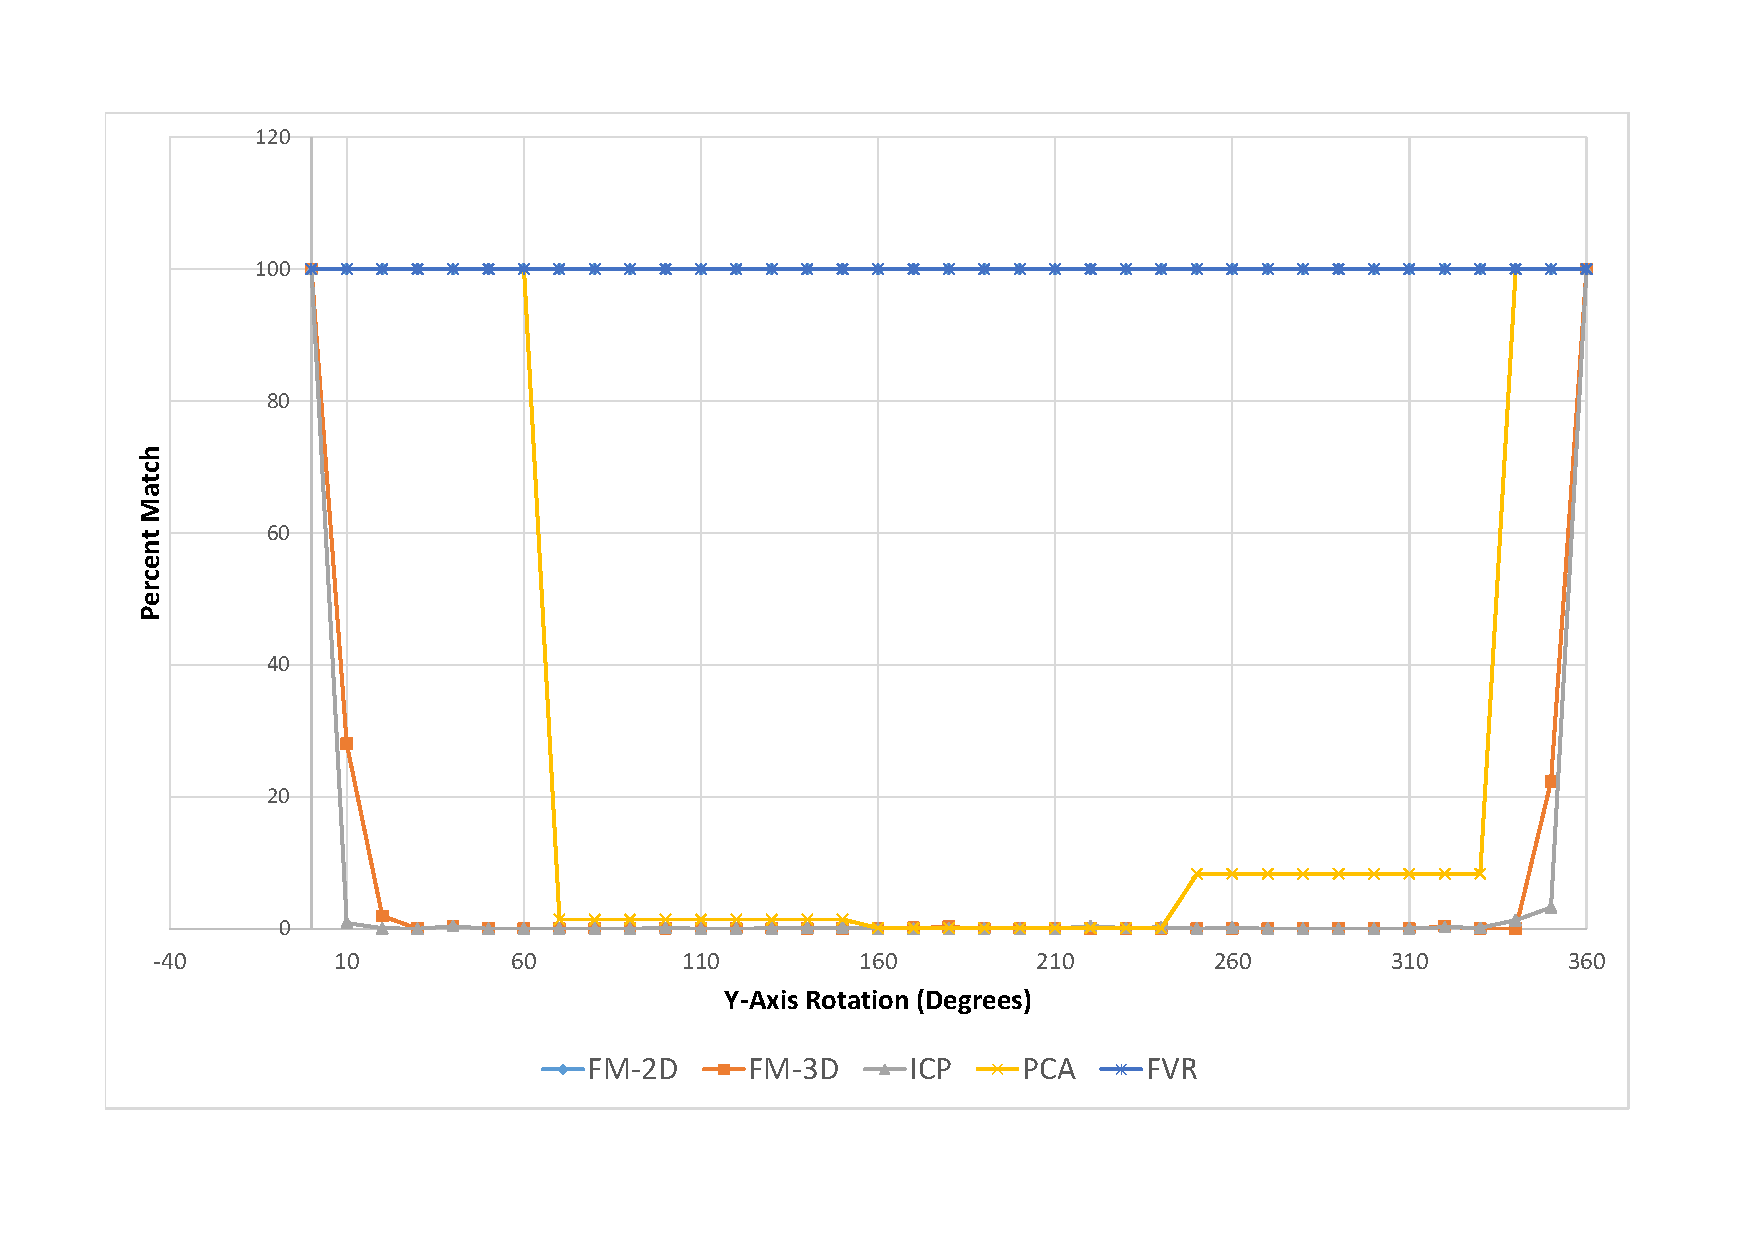
\includegraphics[width=6.0in]{images/results/noise/YRNoise0}
\caption{Percent Match for Y-Axis Registration with an Infinite SNR and noise range of $0$.}
\label{fig:YRNoise0}
\end{figure*}

In the first set of experiments, scanned 3D data was rotated about the Y-axis. Figure \ref{fig:YRNoise0} shows results with an infinite SNR. The 2D-FM method and FVR achieved perfect results. PCA performed next best, but failed to register degrees above 70. Since no noise was present, PCA was truly accurate, however some axes were flipped. This may be fixed by testing the data for flipped axes. FM-3D and ICP fell away much earlier. ICP is not good at registering significant transforms and FM-3D also does not perform well as quantization errors are higher since we use volume sizes of $128^3$.

\begin{figure*}[t]
\centering
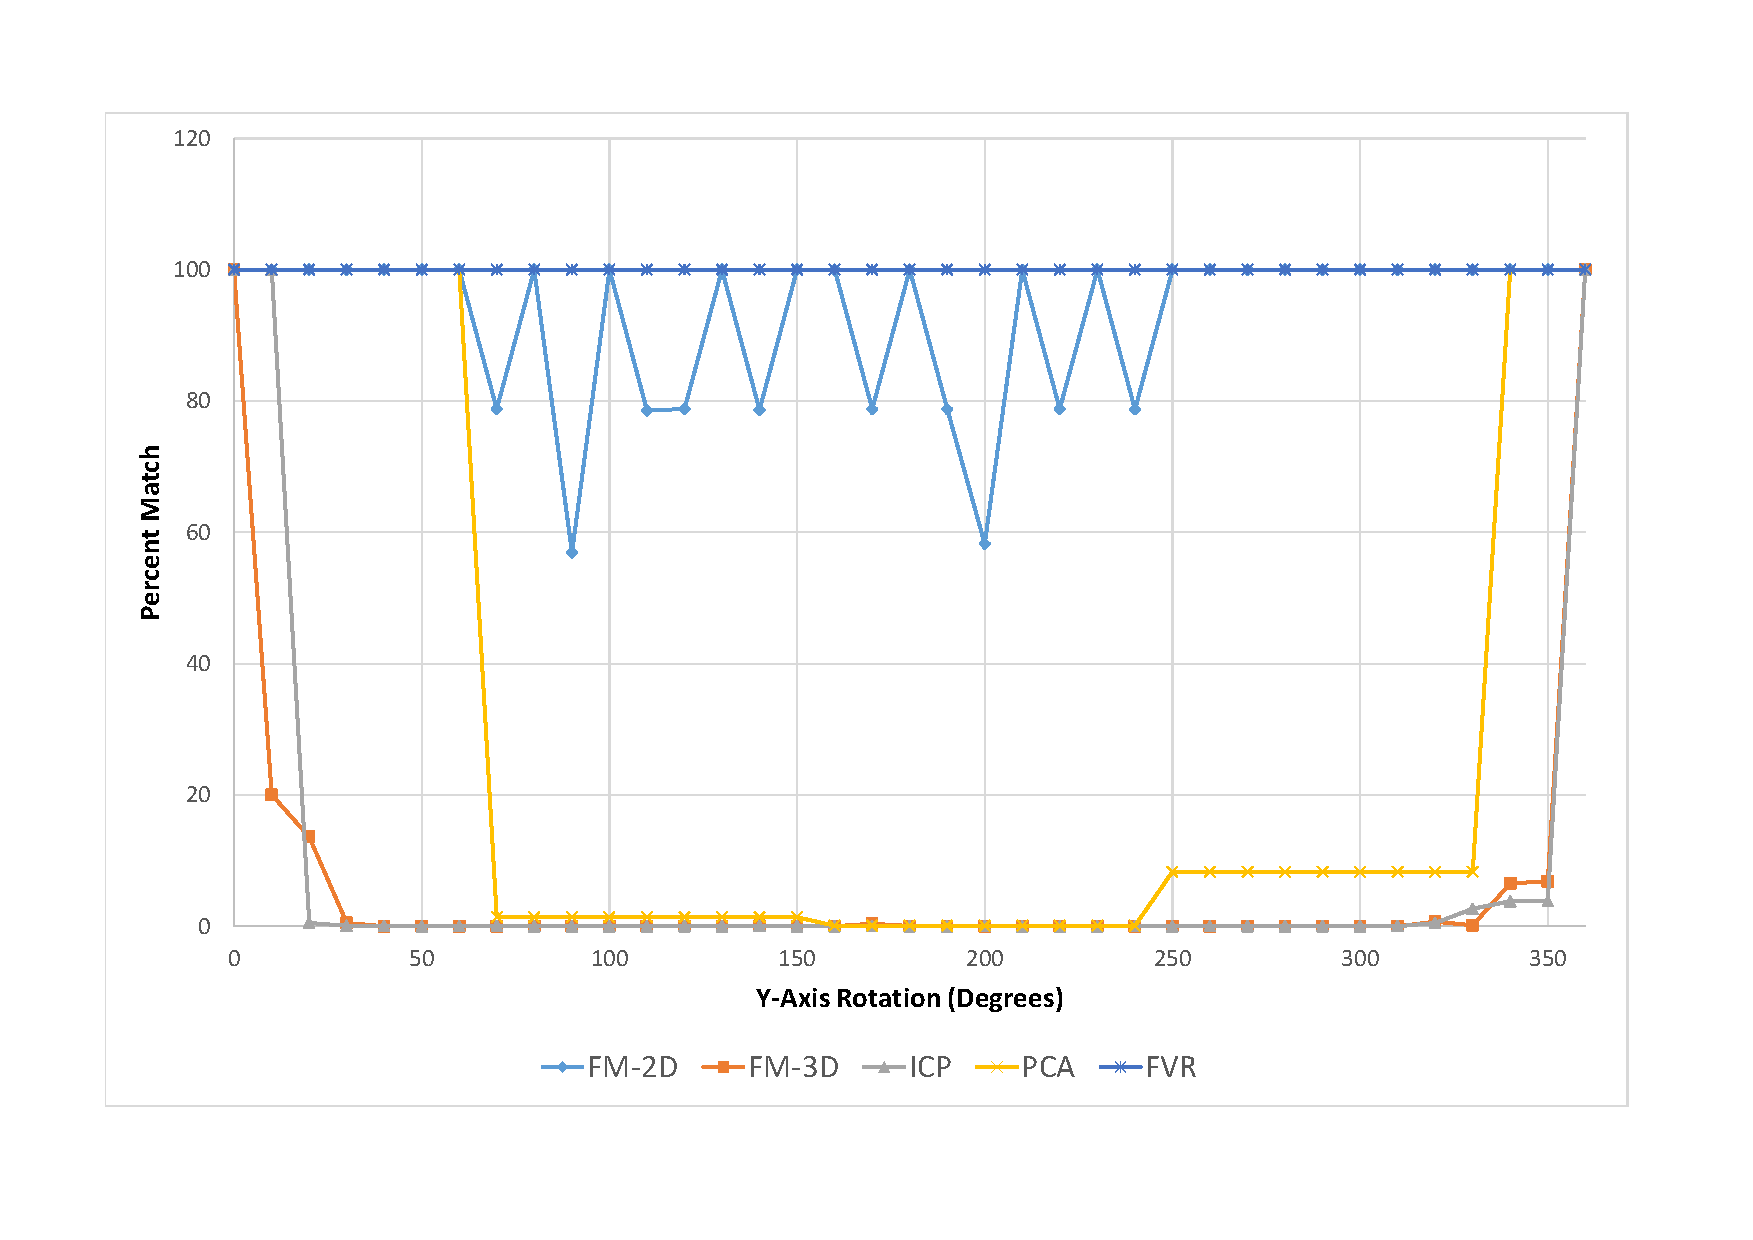
\includegraphics[width=6.0in]{images/results/noise/YRNoise1}
\caption{Percent Match for Y-Axis Registration with an SNR of and noise range of $10300$ and noise range of $1.0$.}
\label{fig:YRNoise1}
\end{figure*}

For the results in figure \ref{fig:YRNoise1} we dropped the SNR to $10300$. Here we see similar results but FM-2D has begun to show some errors with larger rotations (remember rotations above 180 can be considered smaller but negative rotations). In figure \ref{fig:YRNoise2} we reduced the SNR to $2580$ which caused more error in FM-2D. These results suggest that for simple Y-axis rotation, FVR is superior in terms of noise robustness. 

\begin{figure*}[t]
\centering
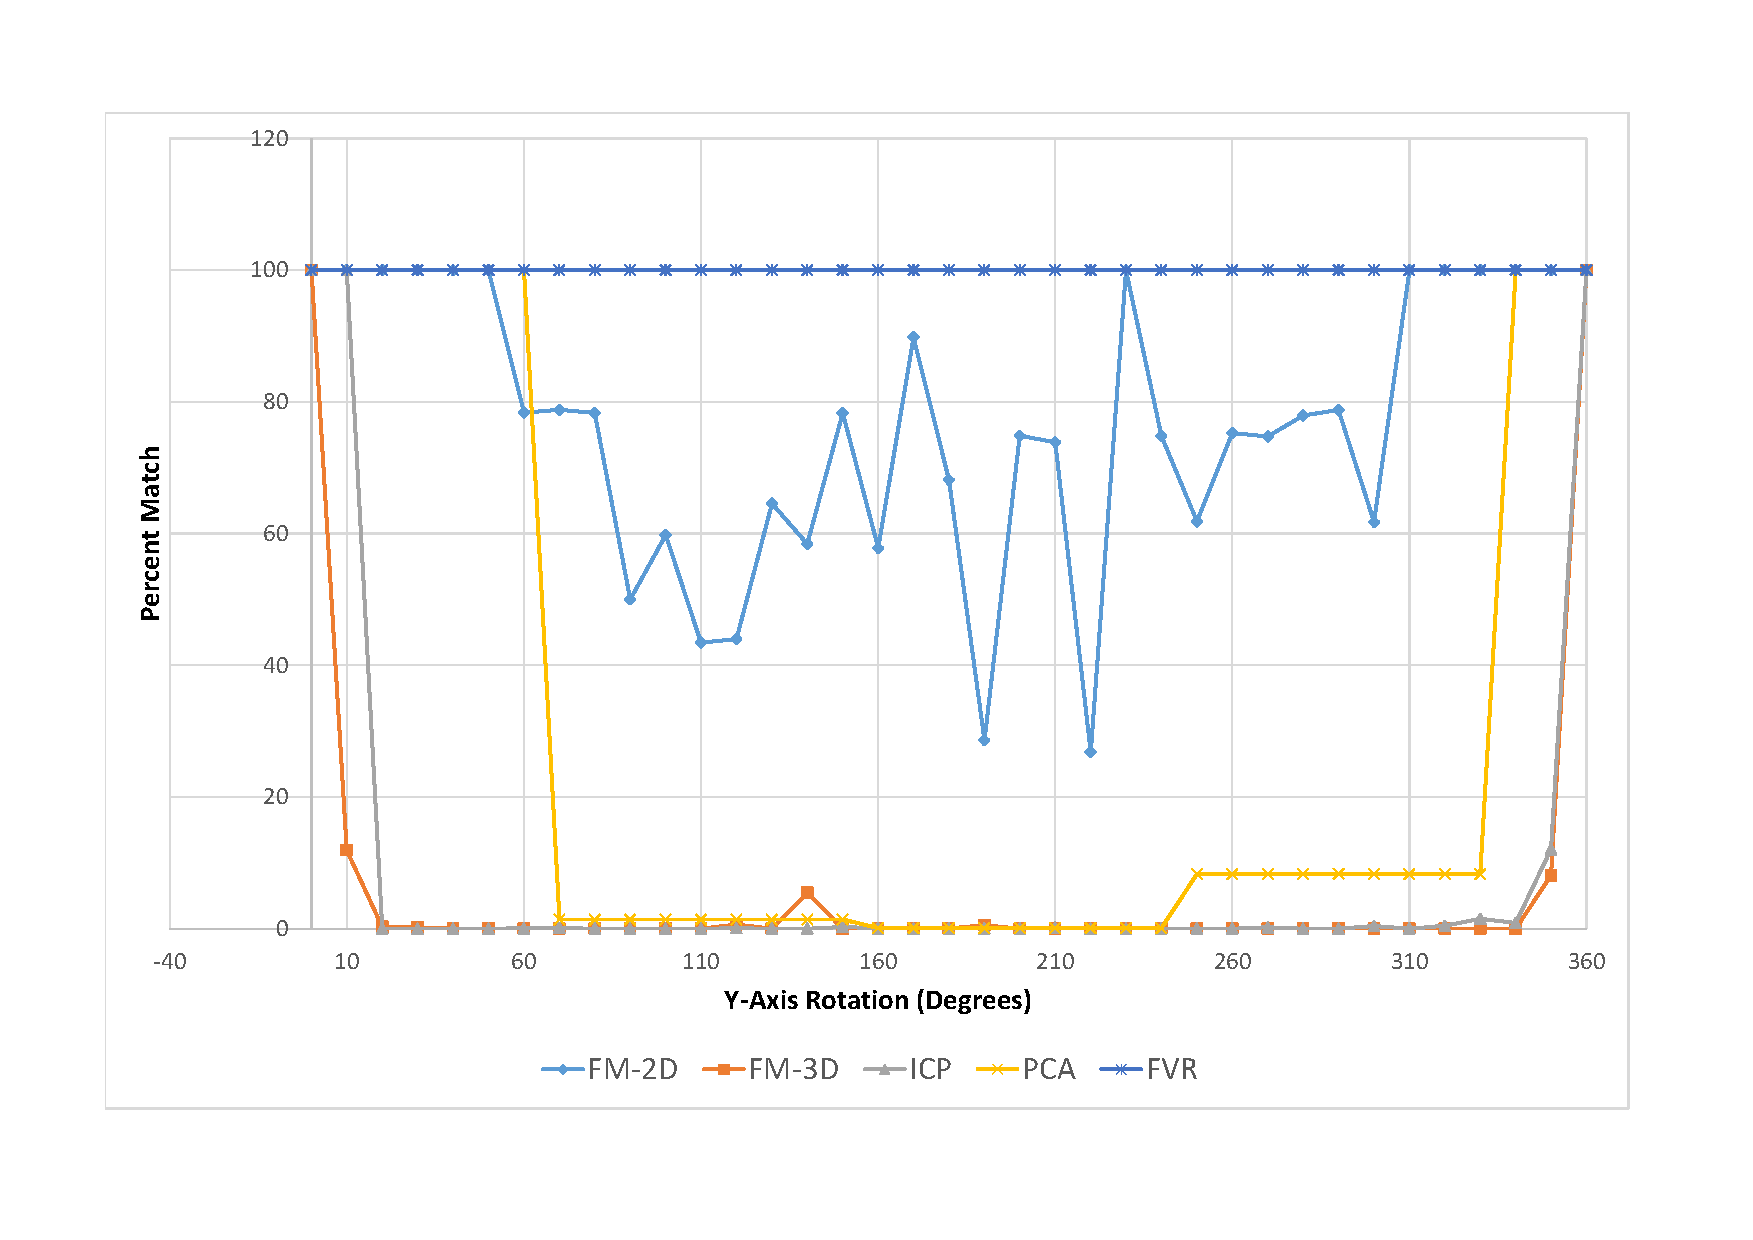
\includegraphics[width=6.0in]{images/results/noise/YRNoise2}
\caption{Percent Match for Y-Axis Registration with an SNR of 2580 and noise range of $2.0$.}
\label{fig:YRNoise2}
\end{figure*}


\begin{figure*}[t]
\centering
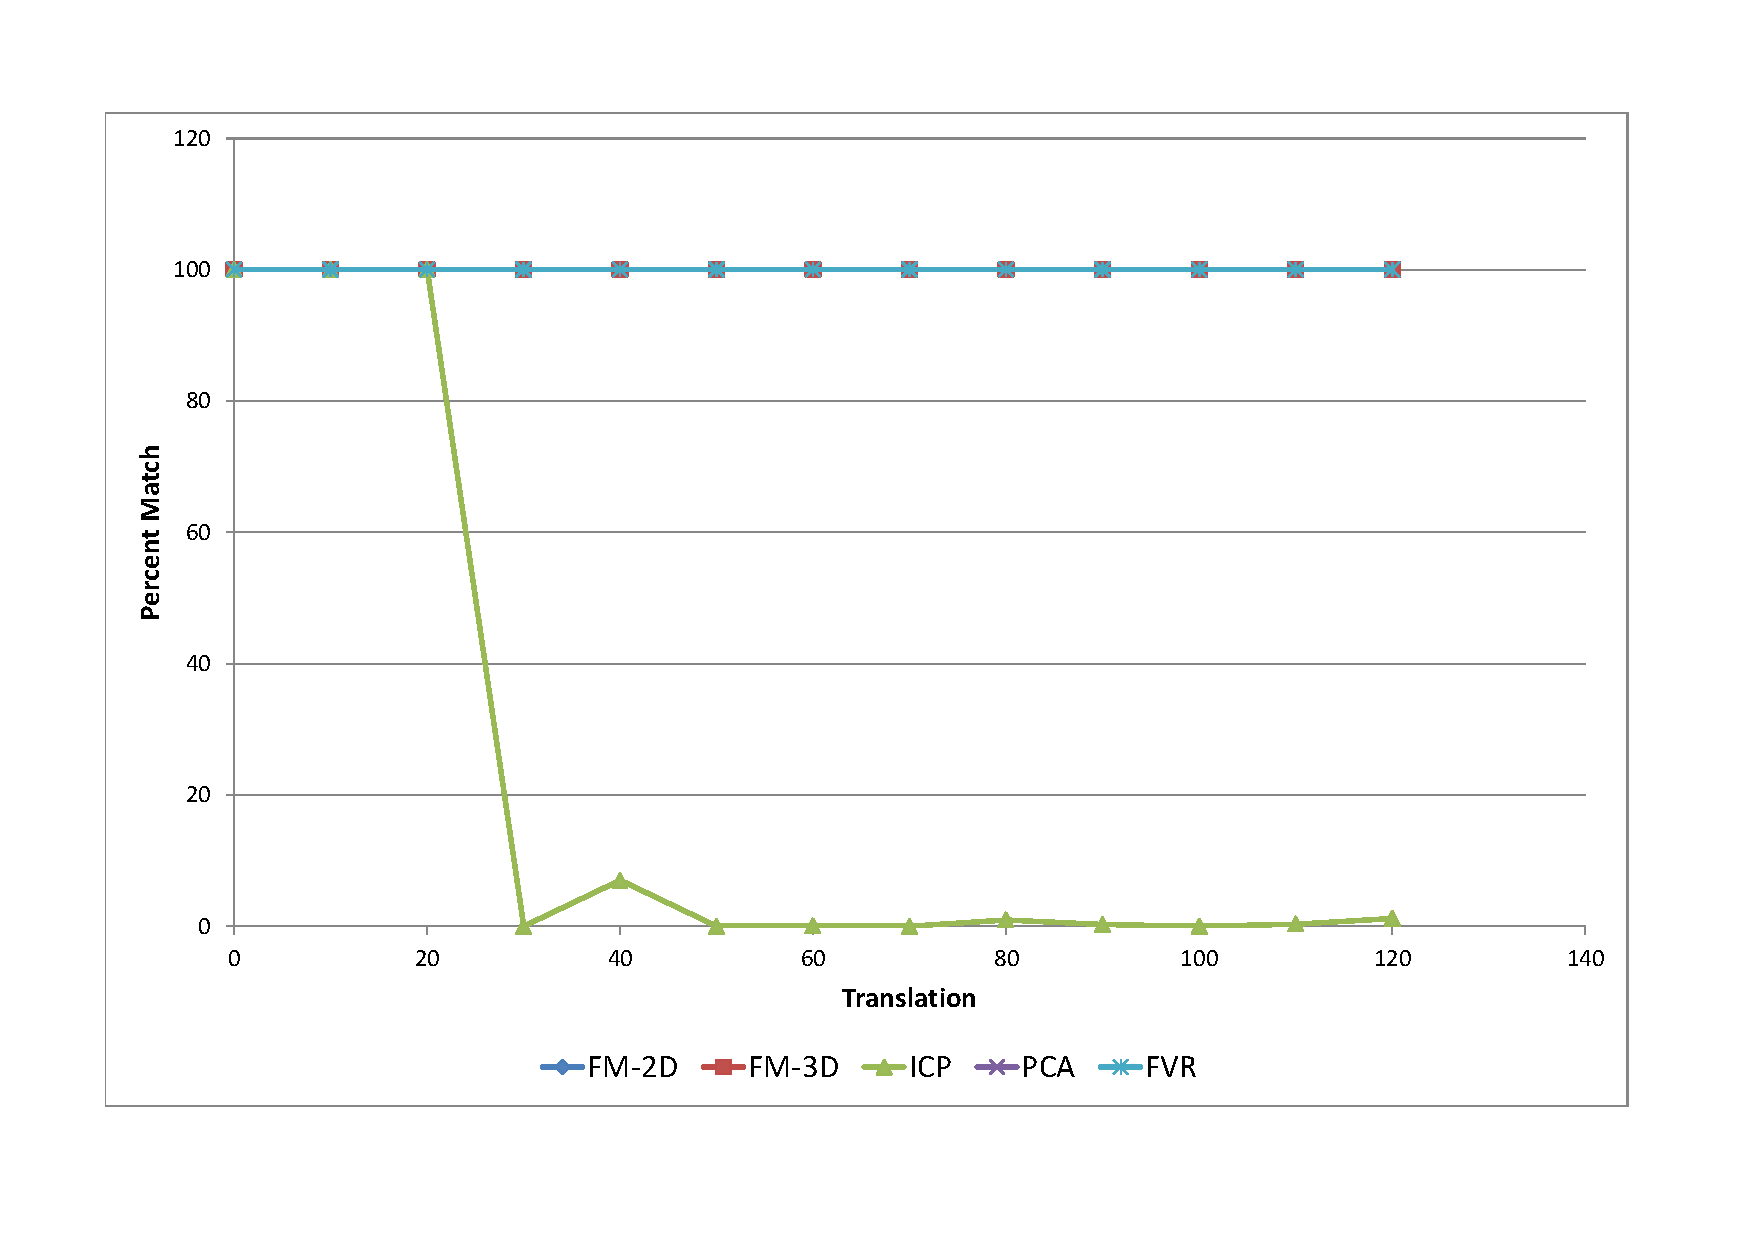
\includegraphics[width=6.0in]{images/results/noise/TransNoise0}
\caption{Percent Match for Translation Registration with an infinite SNR and noise range of $0$.}
\label{fig:TNoise0}
\end{figure*}


\begin{figure*}[t]
\centering
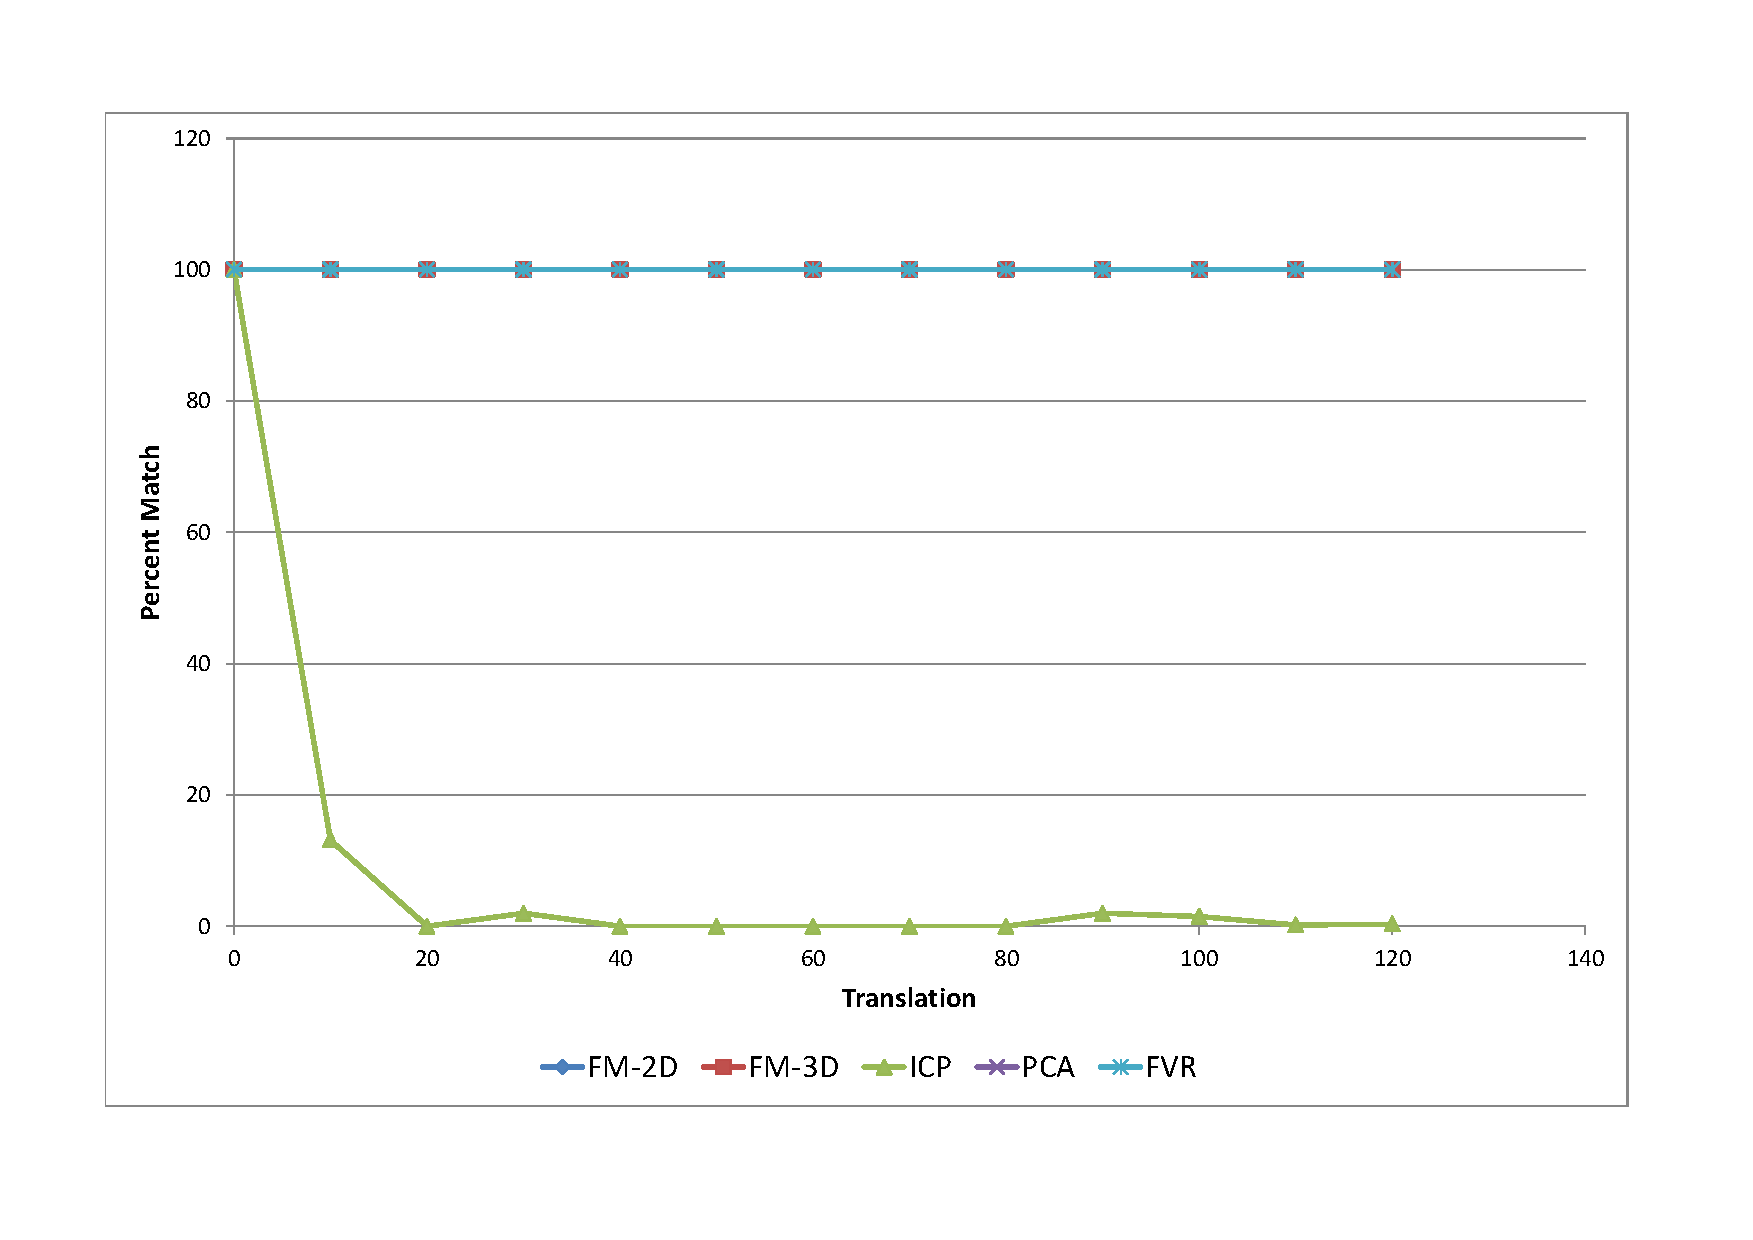
\includegraphics[width=6.0in]{images/results/noise/TransNoise1}
\caption{Percent Match for Translation Registration with an SNR of and noise range of $10300$ and noise range of $1.0$.}
\label{fig:TNoise1}
\end{figure*}


\begin{figure*}[t]
\centering
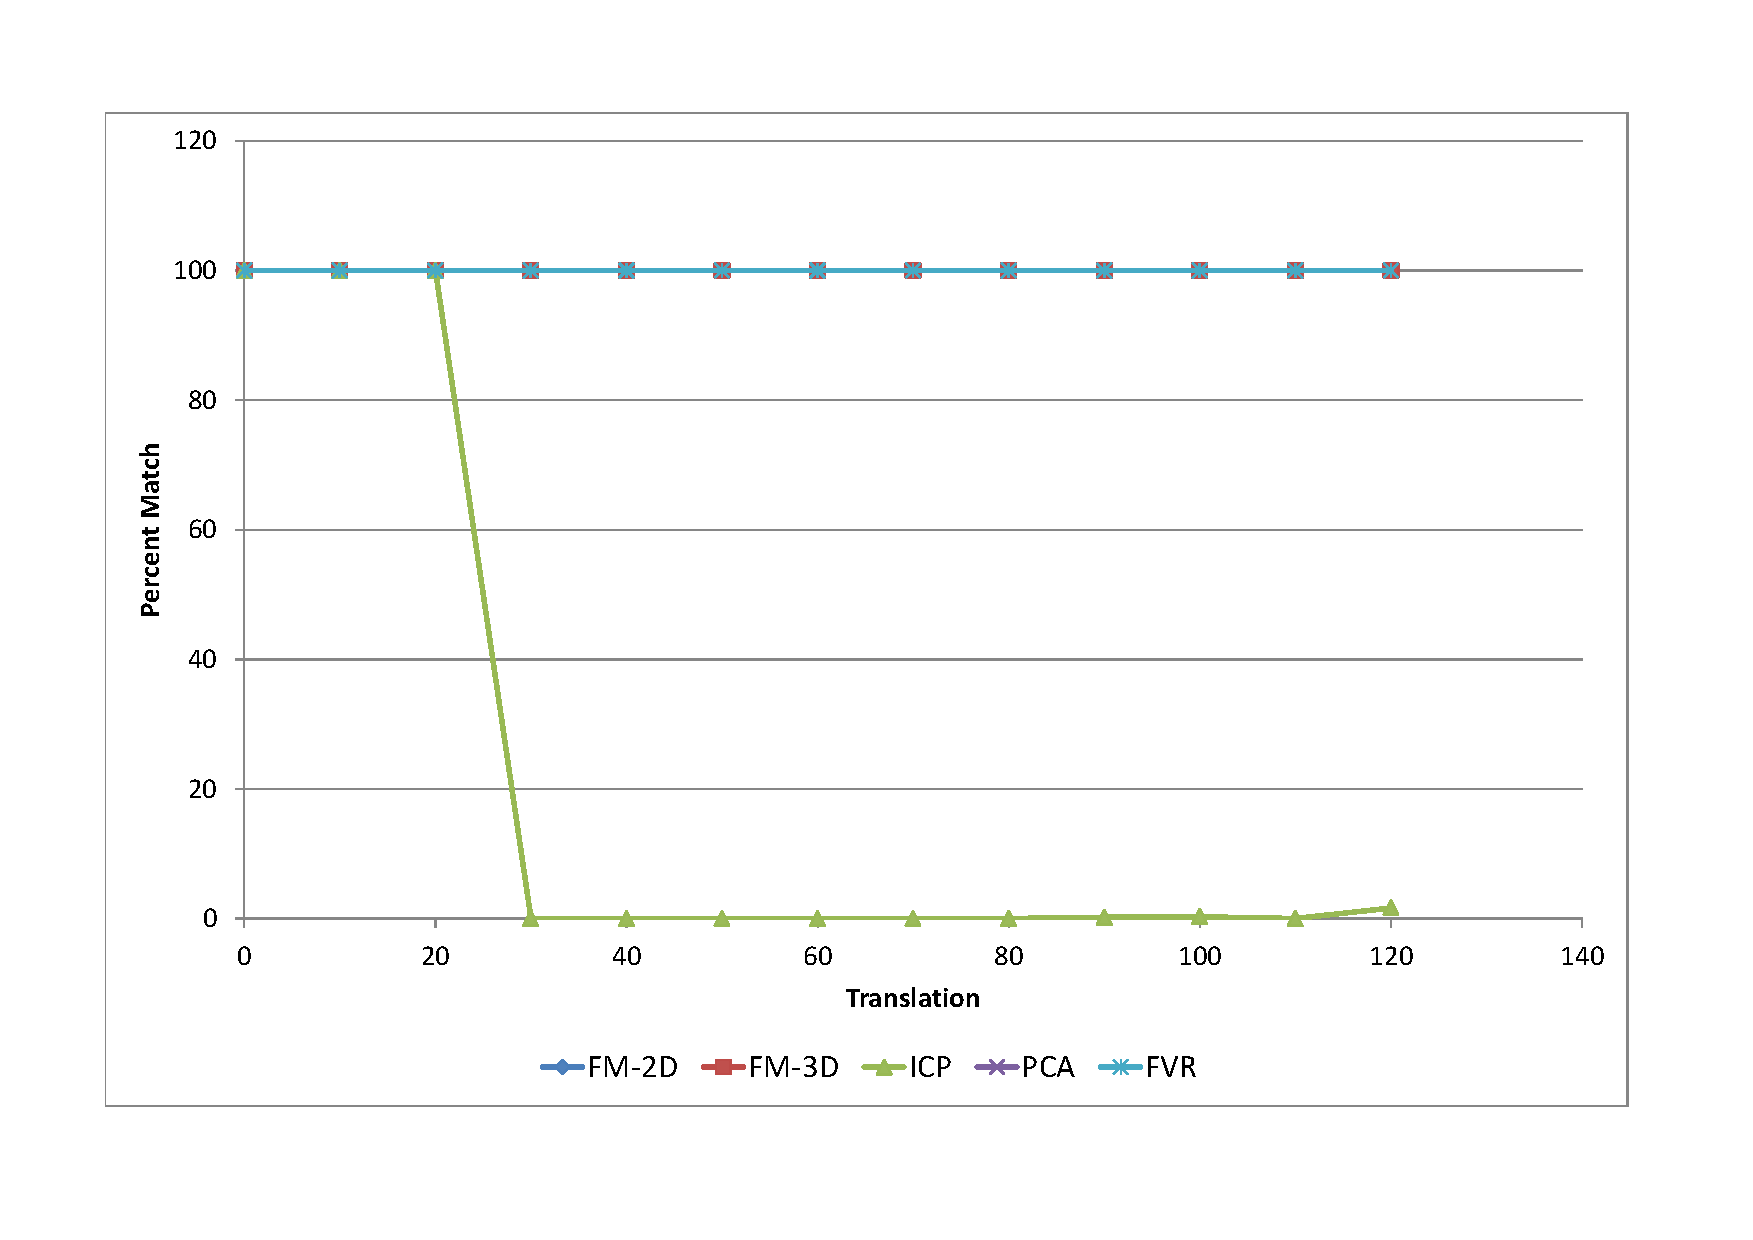
\includegraphics[width=6.0in]{images/results/noise/TransNoise2}
\caption{Percent Match for Translation Registration with an SNR of and noise range of $2580$ and noise range of $2.0$.}
\label{fig:TNoise2}
\end{figure*}
